% This file was converted to LaTeX by Writer2LaTeX ver. 0.5
% see http://www.hj-gym.dk/~hj/writer2latex for more info
\documentclass{article}
\usepackage[ascii]{inputenc}
\usepackage[T1]{fontenc}
\usepackage[english]{babel}
\usepackage{amsmath,amssymb,amsfonts,textcomp}
\usepackage{color}
\usepackage{array}
\usepackage{hhline}
\usepackage{hyperref}
\hypersetup{pdftex, colorlinks=true, linkcolor=blue, citecolor=blue, filecolor=blue, pagecolor=blue, urlcolor=blue, pdftitle=, pdfauthor=qiangwz, pdfsubject=, pdfkeywords=}
\usepackage[pdftex]{graphicx}
% Text styles
\newcommand\textstyleStrongEmphasis[1]{\textbf{#1}}
\newcommand\textstyleCitation[1]{\textit{#1}}
% List styles
\newcommand\liststyleLi{%
\renewcommand\theenumi{\arabic{enumi}}
\renewcommand\theenumii{\arabic{enumii}}
\renewcommand\theenumiii{\arabic{enumiii}}
\renewcommand\theenumiv{\arabic{enumiv}}
\renewcommand\labelenumi{\theenumi.}
\renewcommand\labelenumii{\theenumii.}
\renewcommand\labelenumiii{\theenumiii.}
\renewcommand\labelenumiv{\theenumiv.}
}
\newcommand\liststyleLii{%
\renewcommand\labelitemi{${\bullet}$}
\renewcommand\labelitemii{${\circ}$}
\renewcommand\labelitemiii{${\blacksquare}$}
\renewcommand\labelitemiv{${\bullet}$}
}
\newcommand\liststyleLiii{%
\renewcommand\labelitemi{${\bullet}$}
\renewcommand\labelitemii{${\circ}$}
\renewcommand\labelitemiii{${\blacksquare}$}
\renewcommand\labelitemiv{${\bullet}$}
}
\newcommand\liststyleLiv{%
\renewcommand\theenumi{\arabic{enumi}}
\renewcommand\theenumii{\arabic{enumii}}
\renewcommand\theenumiii{\arabic{enumiii}}
\renewcommand\theenumiv{\arabic{enumiv}}
\renewcommand\labelenumi{\theenumi.}
\renewcommand\labelenumii{\theenumii.}
\renewcommand\labelenumiii{\theenumiii.}
\renewcommand\labelenumiv{\theenumiv.}
}
\newcommand\liststyleLv{%
\renewcommand\theenumi{\arabic{enumi}}
\renewcommand\theenumii{\arabic{enumii}}
\renewcommand\theenumiii{\arabic{enumiii}}
\renewcommand\theenumiv{\arabic{enumiv}}
\renewcommand\labelenumi{\theenumi.}
\renewcommand\labelenumii{\theenumii.}
\renewcommand\labelenumiii{\theenumiii.}
\renewcommand\labelenumiv{\theenumiv.}
}
% Page layout (geometry)
\setlength\paperwidth{8.5in}
\setlength\paperheight{11in}
\setlength\voffset{-1in}
\setlength\hoffset{-1in}
\setlength\topmargin{0.7874in}
\setlength\oddsidemargin{0.7874in}
\setlength\textheight{9.4251995in}
\setlength\textwidth{6.9251995in}
\setlength\footskip{0.0cm}
\setlength\headheight{0cm}
\setlength\headsep{0cm}
% Footnote rule
\setlength{\skip\footins}{0.0469in}
\renewcommand\footnoterule{\vspace*{-0.0071in}\setlength\leftskip{0pt}\setlength\rightskip{0pt plus 1fil}\noindent\textcolor{black}{\rule{0.25\columnwidth}{0.0071in}}\vspace*{0.0398in}}
% Pages styles
\makeatletter
\newcommand\ps@Standard{
  \renewcommand\@oddhead{}
  \renewcommand\@evenhead{}
  \renewcommand\@oddfoot{}
  \renewcommand\@evenfoot{}
  \renewcommand\thepage{\arabic{page}}
}
\makeatother
\pagestyle{Standard}
\title{}
\begin{document}
{\centering
Towards cross-middleware authentication and single sign-on for ARC grid
middleware
\par}


\bigskip

{\centering
Abstract
\par}

\ \ \ \ In order to make the access to Grids as simple as possible,
security is one of the most important challenges in production Grids,
especially when the Grid applications are across multiple
administration domains as well as across heterogeneous Grid
middlewares, such as some wide scale eScience applications which needs
to coordinate resources sharing among collection of autonomous
institutions with different Grid middlewares running on these
resources. In this paper, we describe the security implementation and
consideration in new version of Advanced Resource Connector (ARC)
middleware, where the heterogeneity issue have been exploited. The main
goal of ARC implementation in terms of security is to let the
middleware be capable of interoperating with other Grid middlewares by
leveraging standard specifications. The key aspect of the work we have
done is to enhance the current proxy certificate based authentication
and single sign-on by utilizing and enhancing the standardized Web
Service specifications such as Security Assertion Markup Languages
(\textit{SAML}) single sign-on (SSO) profile, Web Services Security in
order to achieve cross-middleware authentication and single sign-on.


\bigskip

\liststyleLi
\begin{enumerate}
\item[] {\centering
1. Introduction
\par}
\end{enumerate}
\ \ \ \ Grids provides the technology for wide-scale, cross domains
collaboration where the users work on resources and sharing data which
are distributed across domains. This kind of collaboration is called
virtual organization (VO)[1]. The resources that contribute to the VO
could come from independent administrative domains, and even require
different security approaches for control the access to themselves
because different middlerwares are used as platform. The same
heterogeneous situation even critically applies to users who need to
access the VO, because users holding one kind of credential could need
to travel through multiple resources with different security
approaches. To solve the above issues, the Grid middlewares should
provide the following ability: The user which participates the VO
should be able to access data and resources without being required to
constantly do authentication at each resource or data; The VO should be
able to easily manage the privileges or memberships to the users, and
VO together with its resources should be able to easily manage the
authorization, given the condition that the resources are owned by
different administrative domains.

\ \ \ \ In grid community, Grid Security Infrastructure (GSI)[2] is the
\textit{de facto} standard about authentication and \ transport level
communication, which builds on Public Key Infrastructure (PKI), an
architecture based on X.509 public key certificate. GSI implements some
enhancement (such as certificate delegation) based on standard SSL/TLS
protocol. Mutual authentication is required by GSI, and is the default
configuration for GSI based grid deployment; and X.509 certificates is
required for both of the client and service sides in order to achieve
mutual authentication. X.509 certificates is issued by trusted third
party called certificate authorities (CA), and then CAs constitute
trust federation and guarantee two different X.509 certificates from
different CAs can accomplish authentication to each other. So in the
GSI based grid system, if a user would access grid system, he/she
should own a X.509 certificate which is issued by a CA that is trusted
by other entity.

\ \ \ \ In terms of the virtual organization issues mentioned earlier,
GSI and some other related solutions like virtual organization
management service (VOMS) [3] have partly solved the them in some
sense. The identity delegation and X.509 proxy certificate initiated by
GSI can achieve single sign-on, so that the need to re-enter the
user{\textquotesingle}s pass phrase for authentication can be avoided
by creating the proxy certificate. \ As the most successful grid
authorization model, VOMS adopts Attribute Certificate[4]. Attribute
certificate is signed by VOMS server and then binded to proxy
certificates by client, \ and attributes certificate includes the VO
memberships which is associated with the proxy
certificate{\textquotesingle}s identity. Eventually the resources can
make access control decision based on parsing the VO membership
attributes from the homogeneous attribute certificate. 

\ \ \ \ The VO is essentially supposed to be able to provide resource
sharing capability with resources running under heterogeneous
systems/middlewares. This goal can be achieved using Web Service
Architecture (WSA). Therefore, the Web Service technology has been
converged into Grid computing middlewares. The Web Service technology
has been adopted by Globus toolkit[5], gLite[6], as well as \ Advanced
Resource Connector(ARC) [7]. In fact, utilizing Web Service technology
and providing seamless interoperability with other middlewares is one
of the main goals of the new version of ARC middleware.

\ \ \ Unfortunately, the existing grid security solutions such as GSI
and VOMS do not apply to Web Service \ based application very well due
to the following reasons:

\liststyleLii
\begin{itemize}
\item Firstly, \ the GSS API based confidential communication has also
not been adopted by Web Service implementation.
\item Secondly, \ Attribute Certificate has not been adopted by any Web
Service implementation at all.
\item Thirdly, Web Service implementations commonly use the Web Services
Security(WS-Security)[8], Security Assertion Markup Languages
(SAML)[9], and standard SSL/TLS as well as standard X.509 certificate
when considering security, which make them impossible to interoperate
with the GSI based grid middlewares.
\item Finally, identity delegation is a good solution for user or
user{\textquotesingle}s delegatee (on behalf of the user) to
move/travel from one resource to another resource. But since the
identity delegation has been completely coupled with the GSI
confidential communication process, it is not possible for the existing
identity delegation solution to be used by Web Service applications.
\end{itemize}
\ \ \ \ Moreover, the current grid security solutions require each user
to possess a X.509 certificate. But the process to get a certificate
may take quite long time, since the requester needs to be checked and
approved by the Registration Authority (RA) and then the Certificate
Authority (CA) can issue the certificate according to the approval from
RA. Meanwhile the process to use the certificate is also not so easy
for the wider less-IT focused research community to deal with, since
the user need to generate the proxy certificate by using the grid
specific command lines, such as \textit{grid-proxy-init}, and
\textit{voms-proxy-init}. On the other hand, users could most normally
have some local community/institutional credentials such as
username/passwords to which users are more familiar. To enable users to
use their own community credential instead of the X.509 certificate to
access grid is a promising solution to make the grid be more easily
accessible. 

\ \ \ \ The above analysis shows that in order to achieve
interoperability and accessibility for user to access grid system which
is established on different middlewares, we need to address the
mismatch between the different security solutions from these
middlewares in order to ensure the interoperability as wide as
possible; also need to address the mismatch between
user{\textquotesingle}s normal experience and
middleware{\textquotesingle}s requirement in order to ensure the access
as simple as possible.

\ \ \ \ The approach in the new version of ARC is to utilize the
existing Web Service standards, such as SAML and WS-Security, to
achieve the interoperability and accessibility without breaking
existing grid specific security protocols.

\ \ \ \ The rest of this paper is organized as follows: Section 2 shows
the ARC grid middleware, especially the architecture of the new version
of ARC. Section 3 describes the consideration and implementation about
cross-middleware authentication and single sign-on is presented,
including a few solutions implemented for bridging the mismatch in
terms of authentication and single sign-on. Section 4 discusses the
related research, and Section 5 concludes.


\bigskip

{\centering
2. ARC grid middleware 
\par}

\ \ \ \ ARC(Advanced Resource Connector) is an open source grid
middleware solution released under Apache license. ARC middleware
initially aimed at developing a grid middleware which provides
characteristics such as self-organized, fault-tolerant, non-intrusive,
easy-management [10]. \ Now \ the classic version of ARC provides grid
services such as grid job submission and management, resource
characterization, resource aggregation and discovery, basic data
management, integration of grid security solution, etc. Classic ARC has
been deployed and used in production environment, and been one of the
mainly deployed grid middlewares in Europe.

\ \ \ \ The new generation of ARC is based on the functionality and
capabilities of the classic ARC middleware, and it aims at implementing
a service-oriented middleware which will provide higher levels of
resource and user abstracting through well-defined web service
interface [11] in order to provide interoperability with other
service-based grid middlewares, as well as other Web Service compatible
applications.

\ \ \ \ As the key part of the implementation of new ARC middleware,
there is a lightweight Web Service container called Hosting Environment
Daemon (HED) which provides a host place for various services in
application level, as well as a host place for a bunch of modules to
support flexible, interoperatible, and efficient communication
mechanism for building SOAP based Web Services. The whole design of the
HED is built around the idea of flexibility and modularity, which means
for the developer, he can easily concentrate on the application level
Web Service implementation by only using the core minimum amount of
components if he only would do application level development, or he can
easily concentrate on the middleware level implementation such as
supporting another communication protocol or implementing
authentication mechanism by using the core minimum amount of components
and external dependencies; also for the deployer, he can easily
configure and deploy the middleware and application for different kinds
of requirements without being bothered to know much about the
implementation.

{\centering
Figure 1. The architecture of Host Environment Daemon
\par}

\begin{center}
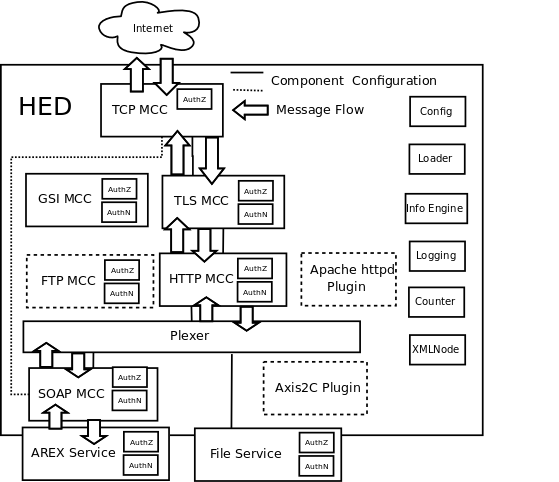
\includegraphics[width=4.0673in,height=3.1047in]{Secpaper-img1.png}
\end{center}
\ \ \ \ The architecture of the HED is illustrated as Figure 1. In
general, there are a few \ components called Message Chain Component
(MCC) which are in charge of processing different messages for
different protocol levels. For instance, as shown in the example
message flow, HTTP MCC will process secure socket stream from TLS MCC
to generate output HTTP message to SOAP MCC, and also process SOAP
documentation from SOAP MCC to generate HTTP message to TLS MCC. 

\ \ \ \ Two examples of MCC components configuration in Figure 1 shows
MCC are flexibly configurable: real line shows SOAP over HTTPS (HTTP
over TLS), while dotted line shows SOAP directly over TCP. Service
administrator can configure the MCCs according to the interoperability
requirement with the other part. For instance, the later example
configuration is compatible to WSE (Web Services Enhancement for .NET)
{\textquotesingle}s SOAP message mechanism (see WSE{\textquotesingle}s
\textit{SoapSender} and \textit{SoapReceiver}). Another configuration
could be SOAP over HTTPG (HTTP over GSI) which can be used to
interoperate with some service based on HTTPG such as Storage Resource
Manager (SRM)[12] \ service. The easily configurable characteristics
shows the flexibility of HED in terms of protocol supporting.

\ \ \ \ HED contains a framework for implementing and enforcing
authentication and authorization. Each MCC or Service has a common
interface for implementing various authentication and authorization
functionality. Each functionality can be implemented as a pluggable and
configurable component (plug-ins) called \textit{SecHandler} which is
C++ class and provides method for processing message that travels
through MCC or Service. Each MCC or Service is usually configured with
two queues of \textit{SecHandler} -- one for incoming message and one
for outgoing message respectively. All \textit{SecHandler} components
attached to the queue are executed sequentially. If any of them fails,
message processing fails as well. In Figure 1, the
{\textquotedblleft}AuthZ{\textquotedblright} and
{\textquotedblleft}AuthN{\textquotedblright} sub-module inside MCCs and
Services are examples of \textit{SecHandler}.

As explained above, HED is supposed to act as a Web/Grid Service
container, but on the client side, from implementation perspective,
there is similar architecture implemented for processing messages from
different protocols and handling security functionality, also there is
a specific application programming interface (API) for developers to
easily write Web Service client code.


\bigskip

{\centering
3. Cross-middleware authentication and Single Sign-On
\par}

\ \ \ \ We exploited the authentication and single sign-on issue in the
scenario that user or user{\textquotesingle}s delegatee (act on behalf
of this user) needs to access across different middlewares. Our work
comprises the following five major aspects:

\liststyleLiii
\begin{itemize}
\item \textit{Integration of community authentication} -{}-{}- to
utilize the standard-compatible community authentication mechanism from
Shibboleth [13] Identity Provider software when users authenticate
against Grid services.
\item \textit{Short lived credential service} \ {}-{}-{}- to issue the
short lived X.509 certificate for user by using the community
authentication, in order to interoperate with services that depends on
PKI based mutual authentication.
\item \textit{Credential delegation service} -{}-{}- to process the
X.509 credential delegation as a normal Web Service, in order to
provide single sign-on characteristic.
\item \textit{Message level authentication} -{}-{}- to provide message
level authentication by implementing WS-Security.
\item \textit{SAML token delegation service} -{}-{}- to process the WS
Security SAML token in order to provide single sign-on for SOAP message
level authentication.
\end{itemize}
3.1 Community based authentication for Grid by utilizing Shibboleth
Identity Provider

\ \ \ \ AAI (Authentication and authorization Infrastructure) is a
solution for the authentication and authorization for
inter-organization resource sharing, such as electronic resource
sharing between libraries, etc. AAI implicitly applies to community or
institutional based authentication where users are from different home
communities but need to get resources from other communities by using
some federation mechanism. Unlike the X.509 based authentication
solution in current grid systems, AAI does not require user to provide
X.509 certificate, instead, it can support different types of
authentication, such as username/password authentication, IP address
authentication, etc. There are a few implementations about AAI, among
which Shibboleth is one implementation which has been widely deployed.

\ \ \ \ Shibboleth provides cross-domain single sign-on and
attribute-based authorization while preserving user privacy. It is
based on the OASIS Security Assertion Markup Language (SAML),
especially the \ new version of Shibboleth supports SAML 2.0
specification. For authentication, the main SAML profile that
Shibboleth implements is the SAML2.0 web browser SSO profile, which
\ define two functional components, an Identity Provider and a Service
Provider. The Identity Provider (IdP) is responsible for creating,
maintaining, and managing user identity, while the Service Provider
(SP) is responsible for controlling access to services and resources by
using the SAML assertion produced and issued by IdP upon request. In
order to discover which home community does a user from, Shibboleth
specifies an optional third component called {\textquotedblleft}Where
Are You From?{\textquotedblright} (WAYF) service to aid in the process
of IdP discovery, and this IdP discovery process is also standardized
and \ defined in SAML 2.0 specification and called as
{\textquotedblleft}Identity Profile Discovery
Profile{\textquotedblright}.

\ \ \ \ We utilized the SAML2.0 web browser SSO profile for the
authentication in ARC middleware. But since the SSO profile is
initially supposed to protect web applications and provide
authentication for web users, we implemented some external code on the
client and service side to integrate SSO profile. On the client side,
apart from the client interface for writing Web Service client, we
implemented the user agent functionality of web browser in order to
mimic its behavior, such as http redirection, cookie processing (In
fact, the implementation of user agent is also based on the client
interface of ARC, specifically, the https client interface, since the
client interface of ARC can support different protocols which are
incarnated by different MCC). Hence client developers who would use
SAML2.0 SSO profile should call the user agent interface and then the
Web Service client interface. On the service side, we implemented the
Service Provider functionality (based on the HTTP MCC configured
together with TLS MCC) which is called SP Service. For Identity
Provider, the Shibboleth IdP implementation is used.

\ \ \ \ Figure 2 shows the process of SAML2.0 SSO integrated in ARC
client and service.



\begin{center}
\includegraphics[width=3.4063in,height=2.1417in]{Secpaper-img2.png}
\end{center}

\bigskip

{\centering
Figure 2. SAML2.0 SSO profile in ARC
\par}

The steps shows in Figure 2 are described as follows:

\liststyleLiv
\begin{enumerate}
\item The client uses the user agent interface to launches a http
request including the IdP name (to which the user belongs) to the
service side. The endpoint of the SP service is the same as that of the
other target services, except the last part of the endpoint is
{\textquotedblleft}saml2sp{\textquotedblright} which is specific for
pointing to the SP Service. Note that we use Identity Provider (IdP)
name here to simplify the IdP discovery process in order to avoid the
IdP discovery process, because we suppose that user who would access
the target services should better know where is he from initially.
\item The SP Service (Service Provider) searches the metadata (we use
the same metadata format defined in Shibboleth) and gets the location
of the single sign-on service (hosted in IdP) and also the location of
assertion consuming service (hosted in this SP itself) in order to
compose the SAML {\textless}\textit{samlp:AuthnRequest}{\textgreater}
message. Then SP Service issues this
{\textless}\textit{samlp:AuthnRequest}{\textgreater} message by using
its own X.509 certificate (Note in the SAML SSO profile, certificate is
still needed by IdP and SP) and sends back to user agent.
\item User agent sends the
{\textless}\textit{samlp:AuthnRequest}{\textgreater} message to
Identity Provider.
\item Identity Provider requires an act of authentication. The
authentication mechanism is outside of the SAML2.0 SSO profile.
Shibboleth IdP implementation chooses some login handler for
authentication. The current user agent implementation is compatible to
\textit{Username/Password} login handler of Shibboleth IdP. Through the
http protocol, user agent will feed IdP with the username/password
which has been given by the caller of user agent interface.
\item Once the authentication has been succeeded, the IdP issues a SAML
response including an encrypted (encrypted by destination
SP{\textquotesingle}s public key) SAML assertion, and then this SAML
response will be delivered by the user agent to the Service Provider. 
\item The SP Service verifies and checks the SAML response, and decrypts
and stores the SAML assertion into session/connection context. The SAML
assertion includes the
{\textless}\textit{saml:AuthnStatement}{\textgreater} and
{\textless}\textit{saml:AttributeStatement}{\textgreater}.
\item The WS client launches the Grid/Web Service request via the same
connection as the one which is used by user agent to contact SP
Service.
\item The Grid/Web Service checks the
{\textless}\textit{saml:AuthnStatement}{\textgreater} from the session
context to see if the session is still valid through the
\textit{SecHandler} called {\textquotedblleft}\textit{SAML
SecHandler}{\textquotedblright}. If valid, service handles the service
processing and returns the response to WS client. Note that service
requires that WS client is from the same connection as the one on which
user agent contact SP service, in order to guarantee that the validity
of SSO profile result effects the WS client/Web Service interaction.
\end{enumerate}
\ \ \ \ The SP service and functional service(s) are hosted by the same
container, and they use the same X.509 credential. The client
authentication is switched off, so that client doesn{\textquotesingle}t
need to use any X.509 credential. Only the trusted certificates (CA
certificates for both SP and IdP) need to be configured for client side
so that SP and IdP can authenticate themselves to the client. As
required by SAML2.0 profile, the SP and IdP should have trust
relationship to each other.

\ \ \ \ One benefit of SAML2.0 SSO profile that is worth mentioning is:
the Identity Provider could cache the authentication result through
session management once the user agent has succeeded to authenticate,
then in a short period this authentication result is valid so that user
agent doesn{\textquotesingle}t need to feed IdP with
user{\textquotesingle}s username and password the next time (if this
point of time is not out of the scope of valid period) it authenticates
against IdP. So user (or the client on behalf of this user) can travel
across multiple security domains with only inputing his name and
password once, which is the characteristic of single sign-on.

\ \ \ \ Since the Shibboleth implementation of SAML is
standard-compliant and widely deployed, the solution implemented in ARC
can easily interoperate with other SAML implementations with minimum
change, and more importantly, this solution can succeed to utilize the
widely deployed SAML implementation for authentication in grid systems
by avoiding the usage of X.509 certificate.

Moreover, even though the implementation is based on ARC middlerware,
the idea can be adopted by other grid middlewares if they only require
server authentication instead of mutual authentication.

3.2 Short-lived credential service

\ \ \ \ However, most of the widely used grid middlewares are based on
GSI while GSI requires mutual authentication. Also for Web Service
based grid solution, we can not prevent service side from requiring
client X.509 certificate. \ Based on the solution described in Section
3.1, we implemented a short lived credential service (SLCS) by which
user can get a short-lived X.509 certificate without being bothered to
contact any registration authority (RA) or certificate authority (CA).

The SLCS service is also a Web Service (standard web service implemented
by using ARC service interface), and the SLCS client is a specific
command-line interface(CLI) which includes the user agent and WS
client. The whole process of SLCS invocation is showed in Figure3 (from
step 1 to step 8), which is the same as in Figure 2, except that step7
and step8 is incarnated for SLCS certificate request and response. 


\bigskip



\begin{center}
\includegraphics[width=3.7689in,height=3.2055in]{Secpaper-img3.png}
\end{center}
{\centering
Figure 3. Short lived credential service
\par}

\ \ \ \ SLCS client generates a X.509 certificate request, launches a
Web Service request which includes the certificate request; SLCS
service then gets the certificate request, composes a distinguished
name (DN), issues a certificate (short lived, 12 hours by default) with
the SAML attribute (from the SAML2.0 SSO profile) as the X.509
certificate extension, and puts the certificate in to the Web Service
response; SLCS client get the response and stores the X.509 certificate
into local repository.

The CLI for the SLCS client is like this:

\$ ./arcslcs -S https://127.0.0.1:60000/slcs -I
https://idp.testshib.org/idp/shibboleth -U myself -P myself

\ \ \ \ Since the lifetime of the short lived credential is normally
short, it is not a must to protect the private key by pass-phrase. As
illustrated in step a and step b in Figure 3, if the private key is not
protected, through Web Service client, the user can use the X.509
certificate to access Grid Service or Web Service from any kind of
middleware. If the private key is protected, the can use the X.509
certificate to generate a proxy certificate (by using command-line
interface utility such as \textit{grid-proxy-init},
\textit{voms-proxy-init}, or \textit{arcproxy}), and then use the proxy
certificate to access Grid Service or Web Service. 

\ \ \ \ It is worth mentioning that since ARC middleware can support GSI
communication by configuring the GSI MCC, \ together with the X.509
certificate, the Web Service client developed by ARC Web Service client
interface can interoperate with Grid Service that requires GSI
communication.

\ \ \ \ It might be noticed that how to compose the distinguished name
(DN) for the certificate is a critical issue for SLCS service. Since
the Shibboleth Identity Provider uses the eduPerson schema [14] for the
definition of {\textless}\textit{saml:Attribute}{\textgreater} in
{\textless}\textit{saml:AttributeStatement}{\textgreater}, we pick the
relatively distinguishable attribute
{\textquotedblleft}\textit{eduPersonPrincipalName}{\textquotedblright}
for the DN. A typical \ \textit{eduPersonPrincipalName} \ value could
be \href{mailto:alice@example.org}{alice@example.org}, then the DN is
{\textquotedblleft}\textit{/O=knowarc/OU=example.org/CN=alice}{\textquotedblright}.

\ \ \ \ The obvious benefit of SLCS service is that: If a user passes
the authentication to his home Identity Provider, he can get the X.509
credential at anywhere only by running the SLCS client command together
with inputing his username and password to this home IdP, and then
access the grid system conveniently; meanwhile, thanks to the single
sign-on characteristic of SAML2.0 SSO profile which is discussed in
Section 3.1, this user doesn{\textquotesingle}t not need to input his
username and password in a valid period after the first time he
succeeds to authenticate against his home IdP by running the SLCS
client command on the same node, even if this SLCS client command is
supposed to run against a few SLCS services to get a few SLCS
credentials.


\bigskip

3.3 X.509 Credential delegation service

\ \ \ \ The delegation of credentials proposed in Grid Security
Infrastructure (GSI) is a good solution for the supporting of single
sign-on for users, except the coupling of the GSI communication which
is not so widely accepted in Web Service applications. In the design of
the new version ARC middleware, we keep the credential delegation idea,
while utilizing the SOAP communication (and TCP or TLS for transport
level communication) instead of the GSI communication for the
credential delegation process.

\ \ \ \ As shown in Figure 4, there is a specific WS client and Web
Service for processing delegation: delegation client, and delegation
service. The delegation service has two main \textit{WSDL}(Web Service
Description Language) operations, one for processing the delegation
initiation; the other for storing the signed proxy certificate. The
delegation process is detailed in Figure 5. 

\ \ \ \ For the service invocation process, the WS client functionality
(inside each service or the initial client) which is included to access
the target service (step a1 or a2 in Figure 4), should use the
user{\textquotesingle}s X.509 certificate or proxy certificate (on
behalf of the user) for authentication and secure communication. For
the delegation process, the principle is the same.

\ \ \ \ Since each WS client accesses the target service (delegation
service or other functional service) on behalf of the user, the trust
relationship between the user{\textquotesingle}s certificates (X.509
certificate and proxy certificate) and services is required, while the
trust relationship between service and service is not required.

 

\begin{center}
\includegraphics[width=3.802in,height=3.0689in]{Secpaper-img4.png}
\end{center}

\bigskip


\bigskip

{\centering
Figure 4. Credential delegation service
\par}


\bigskip



\begin{center}
\includegraphics[width=2.3028in,height=1.6465in]{Secpaper-img5.png}
\end{center}
{\centering
Figure 5. Credential delegation process
\par}

3.4 Message level authentication

\ \ \ \ Transport level security (TLS or SSL) is not sufficient for
securing Web Services, because the secure channel created by SSL/TLS
make it impossible to differentially protect the SOAP message, e.g.
\ to encrypt and/or sign only particular components of the SOAP
message, which is relevant when non-sensitive portions of the message
need to be accessed or changed by intermediate actors. Additionally,
SSL/TLS is incapable of providing end-to-end protection for SOAP
message which might flow through multiple intermediate actors, because
it only allows each hop to be protected with the resultant security
gaps at intermediate actors. Web Services Security (WS-Security)
specification (ref) provides means for applying security to Web
Service.

\ \ \ \ The WS-Security related specifications are implemented in ARC as
\textit{SecHandler}. There are three kinds of WS-Security version 1.1
specifications are completely or partly implemented: Username Token
profile, X.509 Token profile, and SAML Token profile.

\ \ \ \ For those WS clients on behalf of a user, at any step of service
invocation, the WS client can augment the SOAP message with WS-Security
token by simply configuring the WS-Security \textit{SecHandler} into
container{\textquotesingle}s configuration, if the relying party
(target service) requires. 

\ \ \ \ If the WS client owns an X.509 certificate or proxy certificate,
the process of generating an X.509 Token for a SOAP message is: the
client puts the content of certificate into X.509 token as
{\textless}wsse:BinarySecurityToken{\textgreater}, and uses the private
key (corresponding to the certificate) to create XML signature for the
SOAP message body. 

\ \ \ \ However the process of generating a SAML Token is more
complicated. In SAML Token profile, \textit{ConfirmationMethod} is the
verifying method for establishing proof-of-possession for the subject.
Two methods are proposed in SAML Token profile: \textit{holder-of-key},
\textit{sender-vouches}. \ We rely on the \textit{holder-of-key
}method. For the \textit{hold-of-key} subject confirmation method,
there are three interaction parts: the attesting entity, the relying
party and the issuing authority. Firstly the attesting entity
authenticates to issuing authority by using some authentication scheme
such as X.509 Token profile. So then issuing authority is able to make
a definitive statement (sign a SAML assertion) about an act of
authentication that has already taken place. The attesting entity gets
the SAML assertion and then signs the SOAP message together with the
assertion by using its private key (the relevant certificate has been
authenticated by issuing authority, and its relevant public key has
been put into \textit{SubjectConfirmation} 

element under SAML assertion by issuing authority. Only the actual owner
of the SAML assertion can do this, as only the subject possesses the
private key paired with the public key in the assertion. This
establishes an irrefutable connection between the author of the SOAP
message and the assertion describing an authentication event.) 

\ \ \ \ The relying party is supposed to trust the issuing authority.
When it receives a message from the asserting entity, it will check the
SAML assertion based on its predetermined trust relationship with the
SAML issuing authority, and check the signature of the soap message
based on the public key in the SAML assertion without directly trust
relationship with attesting entity (subject owner). 

\ \ \ In terms of verification, since the of proxy certificates has been
introduced in IETF (RFC 3820), \ and OpenSSL has also implemented
RFC3820, it could not be difficult to use the proxy certificate for
X.509 Token profile.


\bigskip

3.5 SAML Token delegation service

\ \ \ \ There is also delegation requirement on the message level, some
entities (client or user) often need to temporarily delegate itself to
another entity to perform action on their behalf. We propose a
delegation mechanism for SAML Token. 

\ \ \ \ The delegation process is similar to the process for delegation
proxy certificate, with the following differences:

\liststyleLv
\begin{enumerate}
\item The communication between delegation client and service is based
on mutual authentication between proxy certificate and service
certificate, instead, it is based on mutual authentication between
service certificate and service certificate.
\item The delegation service will not generate any certificate request,
instead, it picks the public key from its own service certificate, and
sends back to delegation client.
\end{enumerate}
\ \ \ \ Figure 6 shows the SOAP message header is changed due to
delegation. On the left side, B is the identity of the attesting
entity{\textquotesingle}s X509 token mentioned above, while A is the
identity of issuing authority, and the SOAP message is signed by
B{\textquotesingle}s private key. On the right side, C is the identity
of the delegation service (also C is the identity of the target service
\ to which the B will access), and now the SOAP message is signed by
C{\textquotesingle}s private key.


\bigskip



\begin{center}
\includegraphics[width=4.2571in,height=2.152in]{Secpaper-img6.png}
\end{center}
{\centering
\ \ \ \ \ \ \ \ \ Figure 6. SOAP message header with SAML delegation
token inside
\par}


\bigskip

3.6 Discussion


\bigskip


\bigskip

{\centering
4. Related work
\par}


\bigskip

\ \ There is some effort to add GSI support to adapt to the strict
security requirement including GSI from grid middlewares, such as GSI
plug-in for gSOAP[15]. The GSI MCC implemented in ARC can also achieve
the same functionality as gSOAP. Moreover, the ARC solution is flexible
than the gSOAP solution, because both the GSI MCC of service and client
sides are pluggable, which means service and client developer of ARC do
not need to modify the service or client implementation in order to add
or remove the GSI functionality.


\bigskip

Shibboleth

GridShib

gLite Delegation Service?

SWITCH SLCS Service

the CCGrid 06 paper: Shibboleth-Protected privilege management
infrastructure

Delegation service : gridsite


\bigskip


\bigskip

{\centering
5. Conclusion and Future work
\par}


\bigskip


\bigskip

Reference:

[1] Foster I, Kesselman C, Tuecke S. The anatomy of the Grid: Enabling
scalable virtual organizations. International Journal of Supercomputer
Applications 2001; 15(3):200--222. 

\textstyleStrongEmphasis{\textmd{[2]}}\textstyleStrongEmphasis{\textmd{Foster,
I., Kesselman, C., Tsudik, G. and }}Tuecke, S. A Security Architecture
for Computational Grids. ACM Conference on Computers and Security,
1998, 83-91.

[3]R. Alfieri, R. Cecchini, V. Ciaschini, L.
dell{\textquoteright}Agnello, A. Frohner, K. Lorentey, and F. Spataro.
From gridmap- file to voms: managing authorization in a grid
environment. Future Generation Comp. Syst., 21(4):549--558, 2005. 

[4] RFC 3821- An Internet Attribute Certificate Profile for
Authorization. \url{http://www.faqs.org/rfcs/rfc3281.html}

[5] Globus Toolkit. http://www.globus.org/toolkit/

[6]gLite: lightweight middleware for grid computing.
\href{http://glite.web.cern.ch/}{Http://}\href{http://glite.web.cern.ch/}{\textstyleCitation{\textup{glite.web.cern.ch}}}

\textstyleCitation{\textup{[7]Advanced Resource Connector.
}}\url{http://www.nordugrid.org/middleware/}

\textstyleCitation{\textup{[8]Web Services Security(WS-Security).
www.oasis-open.org/committees/wss/}}

\textstyleCitation{\textup{[9]OASIS Security Assertion Markup Languages
(SAML). www.oasis-open.org/committees/security/}}

\textstyleCitation{\textup{[10]}}\textstyleCitation{\textup{M. Ellert,
M. Gr{\o}nager, A. Konstantinov, B. Konya, }}J. Lindemann, I. Livenson,
J. Langgaard Nielsen, M. Niinimaki, O. Smirnova, and A. Waananen.
Advanced resource connector middleware for lightweight computational
grids. Future Generation computer systems, 23(2):219--240, 2007.

\textstyleCitation{\textup{[11] Design document of new version ARC.
}}\url{https://www.knowarc.eu/documents/Knowarc_D1.1-1_07.pdf}

\textstyleCitation{\textup{[12]A. Shoshani, A. Sim, and J. Gu,
}}\textstyleCitation{Storage Resource Managers: Essential Components
for the Grid}\textstyleCitation{\textup{, Grid Resource Management:
State of the Art and Future Trends, Kluwer Publishing, 2003.}}

[13]The Shibboleth Project.
\href{http://shibboleth.internet2.edu/}{Http://shibboleth.internet2.edu/}

[14]eduPerson and eduOrg Object shema.
\url{http://middleware.internet2.edu/eduperson/}

\textstyleCitation{\textup{[15]}}\textstyleCitation{\textup{Giovanni
Aloisio, Massimo Cafaro, Italo Epicoco, Daniele Lezzi, and Robert van
Engelen, }}\textstyleCitation{The GSI plug-in for gSOAP: Enhanced
Security, Performance, and Reliability}\textstyleCitation{\textup{, in
the ITCC conference 2005, IEEE Press, Volume I, pages 304-309.}}


\bigskip


\bigskip


\bigskip
\end{document}
